% 固定来源第1页左栏Q6：四条幂函数曲线及(1,1)对应刻度。
% 依据题中给定四个指数数学化重建，绘图坐标不增加题设。
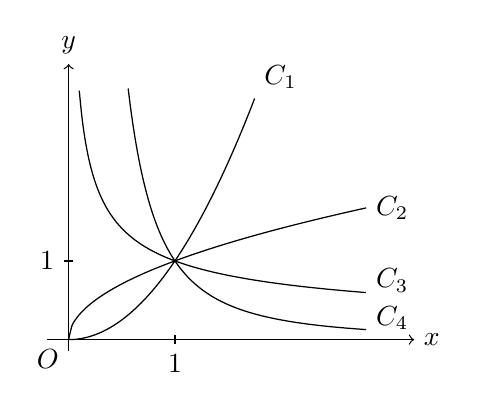
\begin{tikzpicture}[x=1.35cm,y=1.0cm,line width=0.45pt]
  \draw[->] (-0.2,0)--(3.25,0) node[right] {$x$};
  \draw[->] (0,-0.15)--(0,3.5) node[above] {$y$};
  \draw (1,0.06)--(1,-0.06) node[below] {$1$};
  \draw (0.045,1)--(-0.045,1) node[left] {$1$};
  \node[below left] at (0,0) {$O$};
  \draw[domain=0:1.75,samples=70,smooth] plot (\x,{\x*\x});
  \draw[domain=0:2.8,samples=90,smooth] plot (\x,{sqrt(\x)});
  \draw[domain=0.1:2.8,samples=120,smooth] plot (\x,{1/sqrt(\x)});
  \draw[domain=0.56:2.8,samples=120,smooth] plot (\x,{1/(\x*\x)});
  \node[above right] at (1.75,3.0625) {$C_1$};
  \node[right] at (2.8,{sqrt(2.8)}) {$C_2$};
  \node[right] at (2.8,0.75) {$C_3$};
  \node[right] at (2.8,0.27) {$C_4$};
\end{tikzpicture}
